\documentclass[oneside]{book}
\usepackage[a4paper, total={6in, 8in}]{geometry}
\usepackage[italian]{babel}
\usepackage[utf8]{inputenc}
\usepackage[T1]{fontenc}
\usepackage{amsmath}
\usepackage{amsfonts}
\usepackage{listings}
\usepackage{hyperref}
\usepackage{siunitx}
\usepackage{fancyhdr}
\pagestyle{fancy}
\usepackage{textcomp}
\usepackage{makecell}
\usepackage[font=small,labelfont=bf]{caption}
\usepackage{pdfpages}
\usepackage{multicol}
\usepackage[ruled,vlined]{algorithm2e}
\usepackage{mhchem}
\usepackage{float}
\usepackage{graphicx}
\pagestyle{fancy}
\fancyhf{}
\lhead{\rightmark}
\cfoot{\leftmark}
\rfoot{\thepage}

\setcounter{secnumdepth}{5}

\lstset{
    frame=tb, % draw a frame at the top and bottom of the code block
    tabsize=4, % tab space width
    showstringspaces=false, % don't mark spaces in strings
    numbers=none, % display line numbers on the left
    commentstyle=\color{green}, % comment color
    keywordstyle=\color{red}, % keyword color
    stringstyle=\color{blue}, % string color
    breaklines=true,
    postbreak=\mbox{\textcolor{green}{$\hookrightarrow$}\space}
}

\renewcommand{\lstlistingname}{}% Listing -> Algorithm
\renewcommand{\lstlistlistingname}{Algoritmi}% List of Listings -> List of Algorithms
\author{
  Giacomo Fantoni \\
  \small Telegram: \href{https://t.me/GiacomoFantoni}{@GiacomoFantoni} \\[3pt]
  Github: \href{https://github.com/giacThePhantom/AlgoritmiStruttureDati}{https://github.com/giacThePhantom/AlgoritmiStruttureDati}}


\renewcommand*{\listalgorithmcfname}{}
\renewcommand*{\algorithmcfname}{}
\renewcommand*{\algorithmautorefname}{}
\renewcommand{\thealgocf}{}


\title{\Huge \textbf{Introduction to machine learning}}

\author{
  Giacomo Fantoni \\
  \small Telegram: \href{https://t.me/GiacomoFantoni}{@GiacomoFantoni} \\[3pt]
  \small Github: \href{https://github.com/giacThePhantom/intro2ml}{https://github.com/giacThePhantom/intro2ml}}
\begin{document}

	\maketitle
	\tableofcontents
	\chapter{Introduzione}

\section{Definizioni}
Si intende per machine learning lo studio di algoritmi che migliorano autonomamente attraverso l'esperienza.
\`E un campo dell'intelligenza artificiale.
Stravolge il paradigma convenzionale della programmazione: un algoritmo di machine learning infatti prende come input un insieme di dati e risultati in modo da produrre un programma che fornisce un risultato appropriato.
Coinvolge pertanto la scoperta automatica di regolarit\`a nei dati attraverso algoritmi in modo da poter compiere azioni basate su di essi.

\section{Processo}
Il machine learning permette ai computer di acquisire conoscenza attraverso algoritmi che inferiscono e imparano da dati.
Questa conoscenza viene rappresentata da un modello che pu\`o essere utilizzato su nuovi dati.

	\subsection{Il processo di apprendimento}
	Il processo di apprendimento in particolare coinvolge diversi passaggi:
	\begin{multicols}{2}
		\begin{itemize}
			\item Acquisizione dei dati dal mondo reale attraverso dispositivi di misurazione come sensori o database.
			\item Preprocessamento dei dati: filtraggio del rumore, estrazione delle feature e normalizzazione.
			\item Riduzione dimensionale: selezione e proiezione delle feature.
			\item Apprendimento del modello: classificazione, regressione, clustering e descrizione.
			\item Test del modello: cross-validation e bootstrap.
			\item Analisi dei risultati.
		\end{itemize}
	\end{multicols}

\section{Modello}
Un algoritmo di machine learning impara dall'esperienza $E$ in rispetto di una classe di compiti $T$ e di misurazione delle performance $P$, se la $P$ di $T$ aumenta con $E$.
Si nota pertanto come un compito di machine learning ben definito possiede una tripla:
$$<T, P, E>$$
Andiamo a vedere degli esempi:
\begin{itemize}
	\item T: Categorizzazzione delle email come spam, P: Percentuale delle email categorizzate correttamente, E: Database delle parole email, alcune etichettate da umani
\end{itemize}
\section{Deep learning}
Il deep learning \`e un sottoinsieme del machine learning che permette a modelli computazionali composti di multipli strati di imparare la rappresentazione di dati con multipli livelli di astrazione.
Si utilizza pertanto una rete neurale con diversi strati di nodi tra input e output.
Questa serie di strati tra input e output computa caratteristiche rilevanti automaticamente in una serie di passaggi.
Questi algoritmi sono resi possibili da:
\begin{multicols}{2}
	\begin{itemize}
		\item Enorme mole di dati disponibili.
		\item Aumento del potere computazionale.
		\item Aumento del numero di algoritmi di machine learning e della teoria sviluppata dai ricercatori.
		\item Aumento del supporto dall'industria.
	\end{itemize}
\end{multicols}

	\chapter{Machine learning basics}

\section{Introduzione}
Il machine learning permette ai computer di acquisire conoscenza attraverso algoritmi che imparano e inferiscono dai dati.
Tale conoscenza viene rappresentata da un modello che viene poi utilizzato su dati futuri.

	\subsection{Processo di learning}
	Si individua un processo di learning:
	\begin{multicols}{2}
		\begin{itemize}
			\item Acquisizione di dati dal mondo reale attraverso sensori.
			\item Preprocessamento dei dati: eliminazione del rumore, estrazione delle features e normalizzazione.
			\item Riduzione di dimensionalit\`a attraverso selezione e proiezione di features.
			\item Learning del modello: classification, regression, clustering e description.
			\item Test del modello attraverso cross-validation e bootstrap.
			\item Analisi dei risultati.
		\end{itemize}
	\end{multicols}

\section{Dati}
I dati disponibili ad un algoritmo di machine learning sono tipicamente un insieme di esempi.
Questi esempi sono tipicamente rappresentati come un array di features, caratteristiche dei dati di interesse per lo studio in atto.

	\subsection{Training e test set}
	In particolare per questi algoritmi si assume sempre che il training e il test set siano distribuiti secondo variabili indipendenti e identicamente distribuite (\emph{i.i.d})
	La distribuzione $P_{data}$ \`e tipicamente sconosciuta ma si pu\`o campionare, attraverso un modello probabilistico di learning.
	In particolare la distribuzione di probabilit\`a di coppie di esempio e label viene detta data generating distribution e sia il training data che il test set sono generati basandosi su di essa.

\section{Task}
Si intende per task una rappresentazione del tipo di predizione che viene svolta per risolvere un problema su dei dati.
Viene identificata con un insieme di funzioni che possono potenzialmente risolverla.
In generale consiste di una funzione che assegna ogni input $x\in\mathcal{X}$ a un output $y\in\mathcal{Y}$:
$$f:\mathcal{X}\rightarrow\mathcal{Y}\qquad\mathcal{F}_{task}\subset\mathcal{Y^X}$$
La natura di $\mathcal{X},\mathcal{Y}, \mathcal{F}_{task}$ dipende dal tipo di task.

\section{Modello}
Un modello \`e un programma per risolvere un problema.
\`E cio\`e l'implementazione di una funzione $f\in\mathcal{F}_{task}$ che pu\`o essere computata.
Un insieme di modelli formano uno spazio di ipotesi:
$$\mathcal{H}\subset\mathcal{F}_{task}$$
L'algoritmo cerca una soluzione nello spazio di ipotesi.
Esistono diversi tipi di modello:
\begin{multicols}{2}
	\begin{itemize}
		\item Generativi e discriminativi.
		\item Parametrici e non parametrici.
	\end{itemize}
\end{multicols}

	\subsection{Target ideale}
	Il target ideale del modello \`e quello di minimizzare una funzione di errore (generalizzazione)
	$$E(f;P_{data})$$
	Questa funzione determina quanto bene una soluzione $f\in\mathcal{F}_{task}$ fitta dei dati.
	Guida pertanto la selezione della migliore soluzione in $\mathcal{F}_{task}$.
	Pertanto:
	$$f^*\in arg\min\limits_{f\in\mathcal{F}_{task}}E(f;P_{data})$$

	\subsection{Target feasible}
	Si deve restringere il focus sul trovare funzioni che possono essere implementate e valutate in maniera trattabile.
	Si definisce pertanto uno spazio di ipotesi del modello $\mathcal{H}\subset\mathcal{F}_{task}$ e si cerca la soluzione all'interno di quello spazio:
	$$f^*_{\mathcal{H}}\in arg\min\limits_{f\in\mathcal{H}} E(f;P_{data})$$
	Si noti come questa funzione non possa essere computata correttamente in quanto $P_{data}$ \`e sconosciuta.

	\subsection{Target attuale}
	Per trovare il target attuale si deve lavorare su un campione di dati o il training set
	$$\mathcal{D}_n=\{z_1,\dots,z_n\}$$
	Dove
	$$z_i=(x_i,y_i)\in\mathcal{X}\times\mathcal{Y}$$
	$$z_i\sim P_{data}$$
	Pertanto in:
	$$f^*_{\mathcal{H}}\in arg\min\limits_{f\in\mathcal{H}} E(f;P_{data})$$
	$E(f;P_{data})$ \`e il training error.

	\subsection{Funzione di errore}
	Le funzioni di generalizzazione e di training error possono essere scritte in termini di una pointwise loss $l(f;z)$ che misura l'errore che avviene a $f$ su un esempio di training $z$.
	$$E(f;P_{data})=\mathbb{E}_{z\sim P_{data}}[l(f;z)]$$
	$$E(f;\mathcal{D}_n)=\dfrac{1}{n}\sum\limits_{i=1}^nl(f;z_i)$$
	Si nota pertanto come l'algoritmo di learning risolve il problema di ottimizzazione con target:
	$$f^*_\mathcal{H}(\mathcal{D}_n)$$

	\subsection{Tipi di errore}
	\begin{multicols}{2}
		\begin{itemize}
			\item Underfitting il modello non fitta sui dati di training, avviene per mancanza di dati.
			\item Overfitting quando i training data sono rumorosi e il modello li fitta perfettamente, ma impara un modello che si adatta solo su di essi e non fitta dati dal mondo reale.
			\item Estimation error, indotto imparando da un campione di dati.
			\item Approximation error, indotto dallo spazio di ipotesi $\mathcal{H}$.
			\item Irreducible error a causa della variabilit\`a intrinseca.
		\end{itemize}
	\end{multicols}

	\subsection{Stimare l'errore di generalizzazione}
	L'errore di generalizzazione pu\`o essere stimato utilizzando diversi insiemi di training, validation e test.
	Si usa il training set per fare training di un modello, quello di validazione per valutarlo e sistemare i suoi iperparametri e dopo di quello si sceglie il modello migliore che si misura attraverso le performance sul test set.

		\subsubsection{Migliorare la generalizzazione}
		La generalizzazione pu\`o essere migliorata:
		\begin{multicols}{2}
			\begin{itemize}
				\item Evitando di ottenere il minimo sul training error.
				\item Riducendo la capacit\`a del modello.
				\item Cambiando l'obiettivo con un termine di regolarizzazione.
				\item Iniettando rumore nell'algoritmo.
				\item Fermando l'algoritmo prima che converga.
				\item Aumentantdo la quantit\`a di dati.
				\item Aggiungendo pi\`u campioni di training.
				\item Aumentando il training set con trasformazioni.
				\item Combinando predizioni da pi\`u modelli decorrelati o ensembling.
			\end{itemize}
		\end{multicols}

			\paragraph{Regolarizzazione}
			Si intende per regolarizzazione la modifica della funzione di training error con un termine $\Omega(f)$ che penalizza soluzioni complesse:
			$$E_{reg}(f;\mathcal{D}_n)=E(f;\mathcal{D}_n)+\lambda_n\Omega(f)$$


\section{Tipi di learning}

	\subsection{Supervised learning}
	Nel supervised learning vengono dati in input a un modello o predittore un insieme di esempi che possiedono una label.
	Il modello poi impara a creare delle predizioni su un nuovo esempio.

		\subsubsection{Dati}
		Nel caso del supervised learning i dati creano una distribuzione:
		$$p_{data}\in\Delta(\mathcal{X}\times\mathcal{Y})$$

		\subsubsection{Classificazione}
		In un problema di classificazione si trova un insieme finito di label discrete.
		In particolare dato un training set $\mathcal{T} = \{(x_1, u_1),\dots(x_m, y_m)\}$, si deve imparare una funzione $f$ per predirre $y$ dato $x$.
		$f$ sar\`a pertanto:
		$$f:\mathbb{R}^d \rightarrow\{1, 2, \dots, k\}$$
		Dove $d$ \`e la dimensionalit\`a di $x$ e $k$ il numero di labels distinte.

			\paragraph{Task}
			Si deve pertanto trovare una funzione $f\in\mathcal{Y^X}$ che assegna ogni input $x\in\mathcal{X}$ a una label discreta.
			$$f(x)\in\mathcal{Y}=\{c_1,\dots,c_k\}$$

		\subsubsection{Regression}
		Un problema di regressione presenta un insieme di label continue.
		Dato un training set $\mathcal{T}=\{(x_1, y_1),\dots,(x_m,y_m)\}$, si deve imparare una funzione $f$ per predirre $y$ dato $x$.
		$f$ sar\`a pertanto:
		$$f:\mathbb{R}^d\rightarrow\mathbb{R}$$
		Dove $d$ \`e la dimensionalit\`a di $x$.

			\paragraph{Task}
			Si deve trovare una funzione $f(x)\in\mathcal{Y}$ che assegna ogni input a una label continua.

		\subsubsection{Ranking}
		Il ranking \`e un tipo particolare di classificazione in cui una label \`e un ranking.

	\subsection{Unsupervised learning}
	Nel unsupervised learning vengono dati in input a un modello o predittore un insieme di esempi senza label.
	Il modello impara a creare delle predizioni su un nuovo esempio.

		\subsubsection{Dati}
		Nel caso del supervised learning i dati creano una distribuzione:
		$$p_{data}\in\Delta(\mathcal{X})$$

		\subsubsection{Clustering}
		Nel clustering, data $\mathcal{T}=\{x_1, \dots, x_m\}$ si deve trovare la struttura nascosta che intercorre tra le $x$ o i clusters.

			\paragraph{Task}
			Si deve trovare una funzione $f\in\mathbb{N}^{\mathcal{X}}$ che assegna ogni input $x\in\mathcal{X}$ a un indice di cluster $f(x)\in\mathbb{N}$.
			Tutti i punti mappati sullo stesso indice formano un cluster.

		\subsubsection{Dimensionality reduction}
		Nella dimensionality reduction si tenta di ridurre il numero di variabili sotto considerazione ottenendo un insieme di variabili principali.

			\paragraph{Task}
			Si deve trovare una funzione $f\in\mathcal{Y}^\mathcal{X}$ che mappa ogni input di molte dimensioni $x\in\mathcal{X}$ a un output a dimensione minore $f(x)\in\mathcal{Y}$, dove $dim(\mathcal{Y})\ll dim(\mathcal{X})$

	\subsection{Reinforcement learning}
	Nel reinforcement learning un agente impara dall'ambiente interagendo con esso e ricevendo premi per lo svolgimento di azioni particolari.
	In particolare, data una sequenza di esempi o stati e una reward dopo il completamento di tale sequenza si impara a predirre l'azione da svolgere per uno stato o esempio individuale.

\section{Polynomial curve fitting}

	\subsection{Dati}
	L'insieme dei dati $\mathcal{D}_n$ consiste di coppie:
	$$\mathcal{D}_n = \{(x_1, y_1),\dots,(x_n,y_n)\}$$
	I dati sono generati dalla funzione $\sin(2\pi x)$ con del rumore.
	Il training set consiste di $10$ punti: $n = 10$.

	\subsection{Modello e spazio di ipotesi}
	Il modello per il polynomial curve fitting \`e:
	$$f_w(x) = \sum\limits_{j = 0}^M w_jx^j$$
	\`E parametrico, dove i parametri sono $\{w_0,\dots, w_,\}$.
	Lo spazio di ipotesi per $M\in\mathbb{N}$ fissato \`e:
	$$\mathcal{H}_M = \{f_w:w\in\mathbb{R}^M\}$$

	\subsection{Error function}
	La funzione di errore per il polynomial curve fitting consiste della media tra le distanze quadratiche tra la predizione effettuata e l'effettiva label.
	La pointwise loss:
	$$l(f;(x_i,y_i)) = [f(x_i) - y_i]^2$$
	La funzione di errore \`e pertanto:
	$$E(f;\mathcal{D}_n) = \mathbb{E}(l(f;(x_i,y_i))) = \frac{1}{n}\sum\limits_{i=1}^n[f(x_i)-y_i]^2$$

	\subsection{Funzione obiettivo}
	Si ricordi che la funzione obiettivo \`e:
	$$f^*_{\mathcal{H}_M}(\mathcal{D}_n)\in\arg\min\limits_{f\in\mathcal{H}_M}E(f;\mathcal{D}_n)$$
	Equivalente rispetto a $f_{w^*}$ dove:
	$$w^*\in\arg\min\limits_{w\in\mathbb{R}^M}\frac{1}{n}\sum\limits_{i=1}^n[f_w(x_i)-y_i]^2$$
	Si noti come questa richieda la risoluzione di un sistema lineare di equazioni.
	Il cambiamento di $M$ influisce grandemente sull'accuratezza della predizione, andando a determinare casi di overfitting o underfitting.
	Con questo caso particolare si trova la soluzione migliore con $M=3$.

	\subsection{Regolarizzazione}
	Il polynomial curve fitting si regolarizza penalizzando i polinomi con grandi coefficienti:
	$$E_{reg}(f_w;\mathcal{D}_n) = \frac{1}{n}\sum\limits_{i=1}^n[f_w(x_i)-y_i]^2 + \frac{\lambda}{n}||w||^2$$
	Dove $||w||^2 = \sum\limits_{i = 1}^n w_i^2$.

	\chapter{KNN}

\section{Introduzione}
Si possono considerare gli esempi come punti in uno spazio $n$ dimensionale dove $n$ \`e il numero di features.
Per classificare un esempio $d$ si pu\`o mettere a $d$ una label uguale a quella dell'esempio pi\`u vicino a $d$ nel training set.
Questo concetto viene esteso nel $K$-nearest neighbour o \emph{K-NN} in cui per classificare un esempio $d$ si trovano i $k$ esempi pi\`u vicini di $d$ e si sceglie la label in maggior numero tra i $k$ vicini pi\`u prossimi.

\section{Misurare la distanza}
Misurare la distanza tra due esempi \`e specifico al problema, ma un modo possibile \`e la distanza euclidea:
$$D(a,b)=\sqrt{(a_1-b_1)^2+\cdots+(a_n-b_n)^2}$$

\section{Decision boundaries}
I decision boundaries sono posti nello spazio delle features dove la classificazione di un punto o un esempio cambia.
In particolare \emph{K-NN} definisce dei decision boundaries localmente tra le classi.

\section{Il ruolo di $K$}
I fattori che determinano la bont\`a di un algoritmo di machine learning sono la sua abilit\`a di minimizzare il training error e minimizzare il gap tra il training error e il test error.
Questi due fattori corrispondono a underfitting e overfitting.

	\subsection{Underfitting}
	L'underfitting avviene quando il modello non \`e capace di ottenere un valore di errore abbastanza piccolo sul training set.

	\subsection{Overfitting}
	L'overfitting avviene quando il gap tra il training error e il test error \`e troppo grande.

\section{Scelta di $K$}
Il valore di $K$ comprende euristiche comuni come $3, 5, 7$ o un numero dispari per evitare pareggi.
Pu\`o essere scelto utilizzando dati di sviluppo.
Per classificare un esempio $d$ si trovano i $k$ vicini pi\`u prossimi di $d$ e si sceglie la classe pi\`u presente nei $k$ scelti.

\section{Variaizoni di $K$}
Invece di scegliere i $K$ vicini pi\`u prossimi si possono contare tutti gli esempi in una distanza fissata.

	\subsection{\emph{K-NN} pesata}
	Si pu\`o pesare il voto di tutti gli esempi in modo che esempi pi\`u vicini pesino di pi\`u.
	Si usa speso qualche tipo di decadimento esponenziale.

	\chapter{Modelli lineari}

\section{Introduzione}
Alcuni approcci del machine learning fanno delle forti assunzioni riguardo i dati.
Questo avviene in quanto se le assunzioni sono vere si possono raggiungere performance migliori. 
Conoscenza pregressa del dominio ci permette di fare assunzioni sui dati.
In caso contrario l'approccio pu\`o fallire miseramente.
Altri approcci che non fanno molte assunzioni riguardo i dati invece permettono di imparare da dati pi\`u vari ma sono pi\`u proni a overfitting e richiedono pi\`u dati di training.

	\subsection{Bias}
	Il bias di un modello \`e quanto forte le assunzioni del modello sono.
	I classificatori a low-bias fanno delle assunzioni minime riguardo i dati come \emph{k-NN} (che assume unicamente che la vicinanza \`e correlata alla classe) e \emph{DT}, e quindi ci permettono di imparare sempre \emph{qualcosa}.
	I classificatori a high-bias fanno assunzioni forti riguardo ai dati.
	
\section{Linear separability}
L'assunzione strong-bias dei modelli lineari \`e la linear separability, ovvero che in due dimensioni le classi si possano separare attraverso una linea, mentre in dimensioni maggiori da un hyperplane.
Un modello lineare \`e pertanto un modello che assume che i dati sono linearmente separabili. 
	
	\subsection{Definire una linea}
	Ogni coppia di valori $(w_1,w_2)$ definisce una linea attraverso l'origine:
	$$0=w_1f_1+w_2f_2$$
	Si pu\`o inoltre vedere il vettore $\overrightarrow{w}=(w_1, w_2)$ come il vettore dei pesi perpendicolare alla linea.
	Per classificare i punti rispetto alla linea si considera il segno sostituendo i punti a $f_1$ e $f_2$.
	La positivit\`a o negativit\`a indica il lato della linea.
	Avere una linea che attraversa sempre l'origine è limitante, dunque i pu\`o estendere l'equazione con:
	$$a=w_1f_1+w_2f_2$$
	In questo modo la linea interseca l'asse delle $y$ in $a$. \ref{fig:chapter04-00}
	
	\begin{figure}
		\centering
		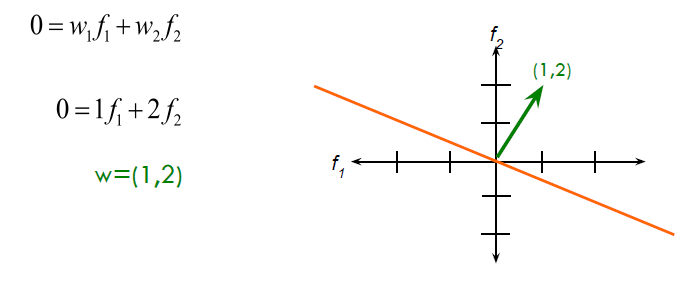
\includegraphics[width=0.6\linewidth]{imgs/chapter4/img0}
		\caption{Definire una linea}
		\label{fig:chapter04-00}
	\end{figure}

\section{Definizione di modello lineare}
Si definisce un modello lineare in uno spazio $n$ dimensionale, dove $n$ \`e il numero di features attraverso $n+1$ pesi.
$$0=b+\sum\limits_{i=1}^nw_if_i$$
In un modello lineare si classifica un nuovo esempio moltiplicandolo con il vettore dei pesi, aggiungendo il bias e controllando il segno del risultato.
Questo determina la classe dell'esempio. 
Siamo dunque interessati alla migliore coppia pesi e bias che separa i dati.

	\subsection{Training}
	Il training di un modello lineare avviene online, ovvero a differenza del modo in batch in cui vengono dati i training data come $\{(x_i, y_i):1\le i\le n\}$, i data points arrivano uno alla volta.
	L'algoritmo allora riceve un esempio $x_i$ senza label, predice la classificazione di questo esempio e confronta la predizione con la risposta corretta $y_i$.
	Infine aggiorna il proprio modello, dunque modifica la linea. 
	Se abbiamo tutti i dati a disposizione possiamo comunque fare training online.
	Le applicazioni del training online sono varie: data streams, dataset di grandi dimensioni, applicazioni che preservano la privacy.
	\subsection{Esempio di training}
	Supponiamo di avere il modello $w=(1,0)$ in figura \ref{fig:chapter04-02}. 
	Abbiamo appena ricevuto un punto in $(-1,1)$, le label ci dicono che quel punto dovrebbe essere classificato come positivo, ma al momento si trova nel lato negativo della linea. 
	Dunque i pesi vanno aggiornati.
	$$w_1*f_1 + w_2 * f_2 = 1 * -1 + 0 * -1 = -1$$
	
	Abbiamo ottenuto un risultato negativo, confermando che i pesi vadano aggiornati, al fine di ottenere un risultato positivo. 
	Possiamo scegliere vari modi per aggiornare i pesi, uno di questi \`e aggiornarli nel seguente modo: $w=(0,1)$, ottenendo il modello in figura \ref{fig:chapter04-03}.
	
	\begin{figure}
		\centering
		\begin{minipage}{.5\textwidth}
			\centering
			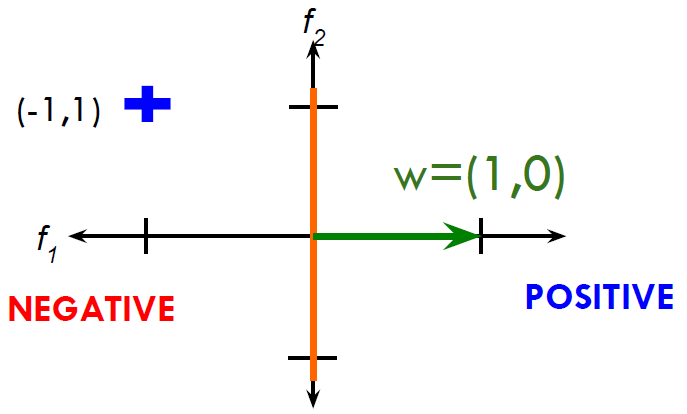
\includegraphics[width=1\linewidth]{imgs/chapter4/img2}
			\caption{Esempio: Modello}
			\label{fig:chapter04-02}
		\end{minipage}%
		\begin{minipage}{.5\textwidth}
			\centering
			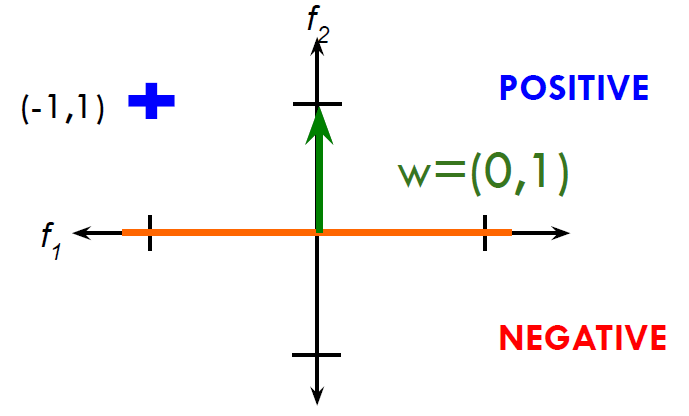
\includegraphics[width=1\linewidth]{imgs/chapter4/img3}
			\caption{Esempio: Modello aggiornato}
			\label{fig:chapter04-03}
		\end{minipage}
	\end{figure}
	
	\subsection{Perceptron}
	\`E un modello parametrico, \`e il blocco di base per la costruzioni di reti neurali.
		\subsubsection{Numero di iterazioni}
		Il numero di iterazioni del perceptron viene deciso in base alla convergenza.
		Inoltre pu\`o essere limitato in modo da ridurre l'overfitting.
		Si noti come in caso di dati non linearmente separabili la convergenza non avviene mai. 
		In caso di dati linearmente separabili abbiamo la garanzia di trovare \textbf{una} linea, non è detto che sia la migliore.
		
		\subsubsection{Ordine dei campioni}
		I campioni da considerare nel perceptron sono considerati in ordine casuale.
		In questo modo si produce un modello a low bias.
		
		\subsubsection{Linear separable sets}
		Le istanze di training sono linearmente separabili se esiste un hyperplane che separa le due classi. \ref{fig:chapter04-01}
		\begin{figure}
			\centering
			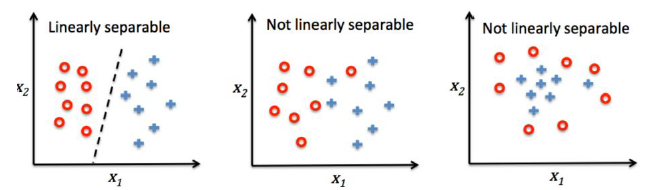
\includegraphics[width=0.6\linewidth]{imgs/chapter4/img1}
			\caption{Linear separable sets}
			\label{fig:chapter04-01}
		\end{figure}
		
		\subsubsection{Algoritmo}
		\begin{algorithm}[H]
\DontPrintSemicolon
\SetKwComment{comment}{$\%$}{}
\SetKw{Int}{int}
\SetKw{To}{to}
\SetKw{Not}{not}
\SetKwData{Item}{item}
\SetKwFunction{Min}{min}
\SetKwFunction{Perceptron}{Perceptron}

\caption{\protect\Perceptron{}}

\Repeat{Convergence}{
	\ForEach{training example ($f_1, f_2,\dots,f_n, label$)}{
		\comment{Label = $\pm 1$}
		check if it is correct based on the current label\;
		\If{\Not correct}{
			\comment{update all the weights}
			\ForEach{$w_i$}{
				$w_i\ =\ w_i\ +\ f_i\ *\ label$\;
				$b\ =\ b\ +\ label$\;
			}
		}
	}
}\comment{Or some number of iteration}



\end{algorithm}

		
		Meglio prendere esempi casuali, perch\`e l'ordine con cui prendiamo gli esempi influenza l'aggiornamento dei pesi.
		
		\subsubsection{Calcolo della predizione}
		\begin{algorithm}[H]
\DontPrintSemicolon
\SetKwComment{comment}{$\%$}{}
\SetKw{Int}{int}
\SetKw{To}{to}
\SetKw{IsNot}{is not}
\SetKw{Not}{not}
\SetKwData{Item}{item}
\SetKwFunction{Min}{min}
\SetKwFunction{Perceptron}{Perceptron}

\caption{\protect\Perceptron{}}

\Repeat{Convergence}{
	\ForEach{training example ($f_1, f_2,\dots,f_n, label$)}{
		\comment{Label = $\pm 1$}
		$prediction\ =\ b\ +\ \sum\limits_{i=1}^nw_if_i$\;
		\If{prediction \IsNot label}{
			\comment{update all the weights}
			\ForEach{$w_i$}{
				$w_i\ =\ w_i\ +\ f_i\ *\ label$\;
				$b\ =\ b\ +\ label$\;
			}
		}
	}
}\comment{Or some number of iteration}



\end{algorithm}


\section{Perceptron e reti neurali}
Si pu\`o immaginare il perceptron come un neurone artificiale o una funzione parametrizzata non lineare con un valore di attivazione soglia e un range di output ristretto.
Le reti neurali sono reti di neuroni artificiali densamente connessi in modo da simulare la rete di neuroni del cervello.

	\subsection{Funzione di attivazione}
	Una funzione di attivazione pu\`o essere una soglia dura: se la somma di tutti gli input \`e maggiore di un valore allora il perceptron manda il segnale queste permettono di imparare solo modelli lineari.
	Funzioni di attivazione pi\`u interessanti sono le sigmoidi, tangenti iperboliche, ReLU o rectified linear unit o leaky ReLU, perch\`e ci permettono di imparare modelli non lineari.
	
	\subsection{Storia del perceptron}
	Il perceptron nasce nel $1958$ da parte di Rosemblatt che lo crea con una soglia dura.
	Questo gli impedisce di imparare modelli non lineari come lo \emph{xor}.
	Viene superato nel $1986$ attraverso perceptrons multi layers e backpropagation e utilizzando una soglia meno dura.

	\chapter{Decision Trees}

\section{Struttura}
Un decision tree \`e un modello di predizione con struttura ad albero.
\`E composto da nodi terminali o foglie e nodi non terminali.
I nodi non terminali hanno da due a pi\`u figli e implementano la funzione di routing.
I nodi foglia non hanno figli e implementano la funzione di predizione.
Non ci sono cicli e tutti i nodi hanno al massimo un genitore (con esclusione del nodo radice).

\section{Funzionamento}
Un decision tree prende un input $x\in\mathcal{X}$ e lo routa attraverso i nodi fino a che raggiunge un nodo foglia dove avviene la predizione \ref{fig:chapter05-00}. 

\begin{figure}
	\centering
	\begin{minipage}{.3\textwidth}
		\centering
		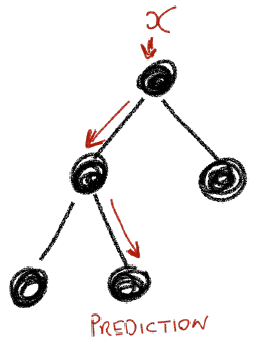
\includegraphics[width=0.7\linewidth]{imgs/chapter5/img0}
		\caption{Funzionamento}
		\label{fig:chapter05-00}
	\end{minipage}%
	\begin{minipage}{.7\textwidth}
		\centering
		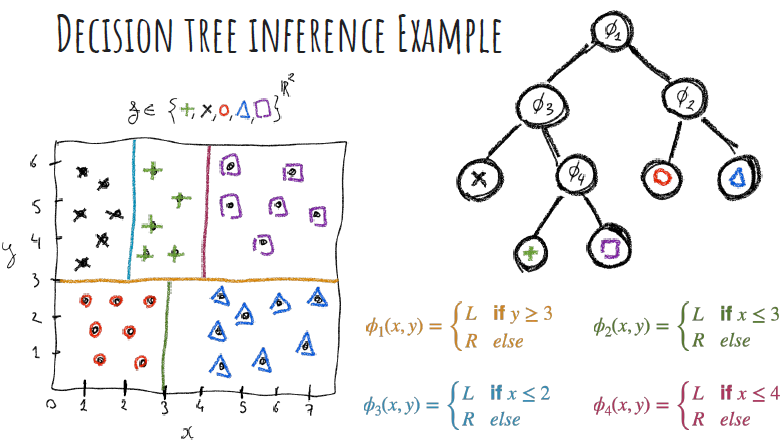
\includegraphics[width=1\linewidth]{imgs/chapter5/img1}
		\caption{Esempio inferenza DT}
		\label{fig:chapter05-01}
	\end{minipage}
\end{figure}

Ogni nodo non terminale
$$Node(\phi, t_L, t_R)$$
Contiene una funzione di routing (decisione) $\phi\in\{L, R\}^{\mathcal{X}}$, un figlio destro $t_L$ e un figlio sinistro $t_R$.
Quando $x$ raggiunge il nodo viene spostato sul figlio destro o sinistro in base al valore di $\phi(x)\in\{L,R\}$.
Ogni nodo foglia
$$Leaf(h)$$
Contiene una funzione di predizione $h\in\mathcal{F}_{task}$, tipicamente una costante. In un problema di classificazione dar\`a in ouput la classe di appartenenza. 
Quando $x$ raggiunge una foglia la previsione finale sar\`a data da: $h(x)$.

	\subsection{Inferenza}
	Sia $f_t$ la funzione che ritorna la predizione per l'input $x\in\mathcal{X}$ secondo il decision tree $t$.
	Questa viene definita ricorsivamente come:
	$$f_t(x)=\begin{cases}h(x)&\mathbf{if}\ t = Leaf(h)\\
		f_{t_{\phi(x)}}(x)&\mathbf{if}\ t = Node(\phi, t_L, t_R)
	\end{cases}$$
	I decision tree dividono lo spazio delle feature in (iper)-rettangoli (consideriamo il caso n-dimensionale), ogni regione rettangolare possiede una label \ref{fig:chapter05-01}.

\section{Decision trees learning algorithm}
Dato un training set $\mathcal{D}_n = \{z_1,\dots, z_n\}$ (dove $z_i$ \`e una coppia $(x,y)$) si deve trovare $f_{t^*}$ dove:
$$t^*\in arg\min\limits_{t\in\mathcal{T}} E(f_t;\mathcal{D}_n)$$
Dove $\mathcal{T}$ \`e l'insieme dei decision trees. 
In parole cerchiamo l'albero che minimizza l'errore.
Il problema di ottimizzazione \`e facile se non si impongono constraints(es: cercare l'albero più compatto), altrimenti potrebbe diventare \emph{NP-hard}.
Una soluzione pu\`o essere trovata utilizzando una strategia greedy.
Pertanto si assume:
$$E(f_t;\mathcal{D}) = \dfrac{1}{|\mathcal{D}|}\sum\limits_{z\in\mathcal{D}}l(f;z)$$
Il training viene svolto in modalit\`a batch.
Ora fissato un insieme di predizioni di foglie
$$\mathcal{H}_{leaf}\subset\mathcal{F}_{task}$$
E fissato un insieme di possibili funzioni di routing o split
$$\Phi\subset\{L,R\}^\mathcal{X}$$
La strategia di crescita dell'albero partiziona ricorsivamente il training set e decide se crescere foglie o nodi non terminali \ref{fig:chapter05-02}. 

\begin{figure}
	\centering
	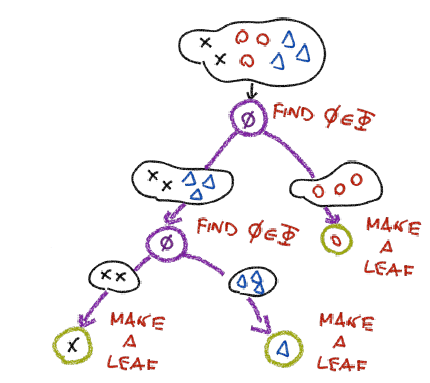
\includegraphics[width=0.4\linewidth]{imgs/chapter5/img2}
	\caption{Decision trees learning algorithm}
	\label{fig:chapter05-02}
\end{figure}


	\subsection{Crescere una foglia}
	Sia $\mathcal{D}=\{z_1, \dots, z_m\}$ il training set che raggiunge un nodo.
	Il predittore di foglia ottimale (con errore minimo) viene computato come:
	$$h^*_\mathcal{D}\in arg\min\limits_{h\in\mathcal{H}_{leaf}} E(h; \mathcal{D})$$
	Il valore di errore ottimale o misura di impurit\`a \ref{fig:chapter05-03}:
	$$I(\mathcal{D}) = E(h^*_\mathcal{D};\mathcal{D})$$
	Dove $h_\mathcal{D}$ \`e la predizione per il dataset $\mathcal{D}$.
	L'impurit\`a \`e computata nel nodo in cui arriva il sottoinsieme del dataset originale $\mathcal{D}$.
	In quel nodo si calcola il numero di errori che si farebbero classificando tutti i dati del sottoinsieme in una singola classe $c$, ripetendo il calcolo per ogni classe.
	Il numero minimo di errori che fai con una certa classe $c^*$ \`e la misura di impurit\`a del classification error.
	Se si raggiungono dei criteri si cresce una foglia $Leaf(h^*_\mathcal{D})$
	Esempi di questi criteri sono la purezza $I(\mathcal{D}) < \epsilon$, la cardinalit\`a minima $|\mathcal{D}|<k$ o un'altezza massima dell'albero.
	
	\begin{figure}
		\centering
		\begin{minipage}{.5\textwidth}
			\centering
			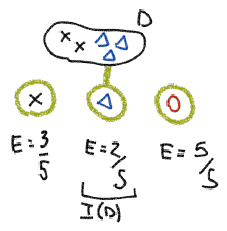
\includegraphics[width=0.6\linewidth]{imgs/chapter5/img3}
			\caption{Misura d'impurit\`a}
			\label{fig:chapter05-03}
		\end{minipage}%
		\begin{minipage}{.5\textwidth}
			\centering
			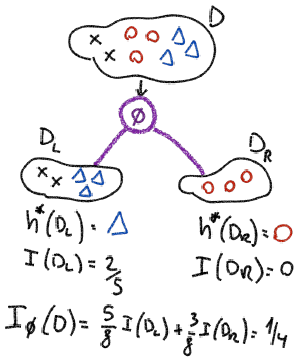
\includegraphics[width=0.6\linewidth]{imgs/chapter5/img4}
			\caption{Crescere di un nodo}
			\label{fig:chapter05-04}
		\end{minipage}
	\end{figure}
	
	\subsection{Crescere un nodo}
	Se non si raggiunge il criterio per creare una foglia si deve trovare una funzione di split ottimale:
	$$\phi^*_\mathcal{D}\in arg\min\limits_{\phi\in\Phi}I_\phi(\mathcal{D})$$
	L'impurit\`a $I_\phi(\mathcal{D})$ di una funzione di split $\phi$ dato il training set $\mathcal{D}$ viene computata nei termini di impurit\`a dei dati splittati:
	$$I_\phi(\mathcal{D})=\sum\limits_{d\in\{L,R\}}\dfrac{|\mathcal{D}^\phi_d|}{|\mathcal{D}|}I(\mathcal{D}^\phi_d)$$
	Dove
	$$\mathcal{D}^\phi_d = \{(x, y)\in\mathcal{D};\phi(x)=d\}$$
	L'impurit\`a di una funzione di split \`e il pi\`u basso errore di training che pu\`o essere ottenuto da un albero che consiste di una radice e due figlie.
	Si cresce pertanto un nodo $Node(\phi^*, t_L, t_R)$ dove $\phi^*$ \`e lo split ottimale, mentre $t_L$ e $t_R$ sono ottenuti applicando ricorsivamente l'algoritmo di learning ai training set splits \ref{fig:chapter05-04}. 
	
	\subsection{Algoritmo}
	$$Grow(\mathcal{D})=\begin{cases}Leaf(h^*_\mathcal{D}) &raggiunto\ criterio\ di\ stop\\
		Node(\phi^*_\mathcal{D}, Grow(\mathcal{D}^*_L), Grow(\mathcal{D}^*_R)) &altrimenti
	\end{cases}$$
	Dove $\mathcal{D}^*_d=\{(x, y)\in\mathcal{D};\phi^*_\mathcal{D}(x)=d\}$.
	
	\subsection{Split selection}
	Tipicamente la migliore funzione di split viene data in termini di minimizzazione dell'impurit\`a dello split, ma altre volte nella massimizzazione del guadagno di informazioni:
	$$\Delta_\phi(\mathcal{D})=I(\mathcal{D})-I_\phi(\mathcal{D})$$
	Essendo $\Delta_\phi(\mathcal{D})\ge 0$ per ogni $\phi\in\{L,R\}^{\mathcal{X}}$ e ogni training set $\mathcal{D}\subset\mathcal{X}\times\mathcal{Y}$, l'impurit\`a non aumentera mai per ogni split scelto casualmente. 
	$\Delta_\phi(\mathcal{D})$ \`e chiamato anche \emph{information gain}.
	
	\subsection{Predizione delle foglie}
	La predizione delle foglie fornisce una soluzione a un problema semplificato coinvolgendo solo dati che la raggiungono.
	Questa soluzione pu\`o essere una funzione arbitraria $h\in\mathcal{F}_{task}$, ma in pratica si restringe a un sottoinsieme di $\mathcal{H}_{leaf}$.
	Il predittore pi\`u semplice \`e una funzione che ritorna una costante (come una label).
	L'insieme di tutte le possibili funzioni costanti pu\`o essere scritto come:
	$$\mathcal{H}_{leaf} = \bigcup\limits_{y\in\mathcal{Y}}\{y\}^{\mathcal{X}}$$

\section{Misure di impurit\`a per la classificazione}
Si consideri per la classificazione:
$$\mathcal{Y} = \{c_1,\dots,c_k\}\qquad\qquad\qquad\mathcal{D}\subset\mathcal{X}\times\mathcal{Y}$$
Sia $\mathcal{D}^y = \{(x, y')\in \mathcal{D}: y = y'\}$, che denota il sottoinsieme di training samples in $\mathcal{D}$ con label $y$.
Considerando la funzione di errore:
$$E(f,\mathcal{D}) = \dfrac{1}{|\mathcal{D}|}\sum\limits_{z\in\mathcal{D}}l(f;z)$$
Se $l(f;(x,y))=1_{f(x)\neq y}$ e $\mathcal{H}_{leaf} = \bigcup\limits_{y\in\mathcal{Y}}\{y\}^\mathcal{X}$ la misura di impurit\`a \`e allora il classification error:
$$I(\mathcal{D})= 1 -\max\limits_{y\in\mathcal{Y}}\dfrac{|\mathcal{D}^y|}{|\mathcal{D}|}$$
Se invece $l(f;(x,y))=\sum\limits_{x\in\mathcal{Y}}[f_c(x)-1_{c=y}]^2$ e $\mathcal{H}_{leaf}=\bigcup\limits_{\pi\in\Delta(\mathcal{Y})}\{\pi\}^\mathcal{X}$ allora la misura di impurit\`a \`e l'impurit\`a di Gini:
$$I(\mathcal{D}) = 1-\sum\limits_{y\in\mathcal{Y}}\biggl(\dfrac{|\mathcal{D}^y|}{|\mathcal{D}|}\biggr)^2$$
Infine se $l(f;(x,y))=-\log f_y(x)$ e $\mathcal{H}_{leaf} = \bigcup\limits_{\pi\in\Delta(\mathcal{Y})}\{\pi\}^\mathcal{X}$, con una distribuzione costante di label come predizione di foglie, allora la misura di impurit\`a \`e l'entropia:
$$I(\mathcal{D})=-\sum\limits_{y\in\mathcal{Y}}\dfrac{|\mathcal{D}^y|}{|\mathcal{D}|}\log\dfrac{|\mathcal{D}^y|}{|\mathcal{D}|}$$

	\subsection{Esempio applicazione dell'algoritmo}
	\begin{multicols}{2}
		\begin{itemize}
			\item Problema di classificazione.
			\item Ottimizziamo l'errore di classificazione.
			\item Le foglie avranno una funzione di predizione che in output d\`a una costante.
			\item Le funzioni di split saranno a una dimensione.
			\item Ci fermeremo (creando una foglia) quando l'impurit\`a avr\`a raggiunto $0$.
		\end{itemize}
	\end{multicols}
	Osserviamo in figura \ref{fig:chapter05-09} come i triangoli siano i pi\`u comuni, dunque  $$I(\mathcal{D})= 1 -\max\limits_{y\in\mathcal{Y}}\dfrac{|\mathcal{D}^y|}{|\mathcal{D}|} = \frac{24}{32} > 0$$
	Poich\`e non \`e stato raggiunto il criterio per crescere una foglia, creiamo un nodo. 
	Prima per\`o dobbiamo capire qual'\`e lo split migliore \ref{fig:chapter05-10}. 
	Lo split a sinistra \`e il migliore in quanto ha l'impurit\`a pi\`u piccola. 
	Il risultato finale \`e in figura \ref{fig:chapter05-11}.
	\begin{figure}
		\centering
		\begin{minipage}{.4\textwidth}
			\centering
			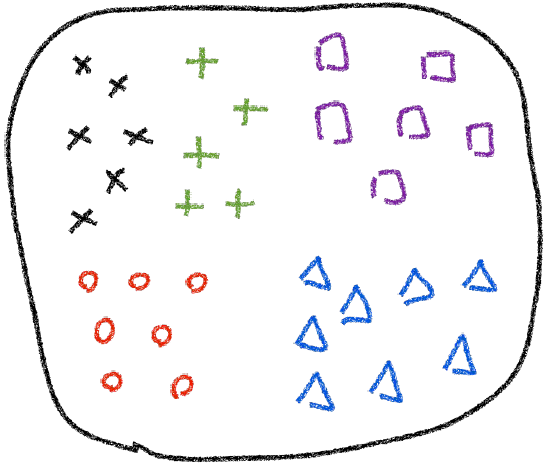
\includegraphics[width=0.8\linewidth]{imgs/chapter5/img9}
			\caption{Punto di partenza}
			\label{fig:chapter05-09}
		\end{minipage}%
		\begin{minipage}{.6\textwidth}
			\centering
			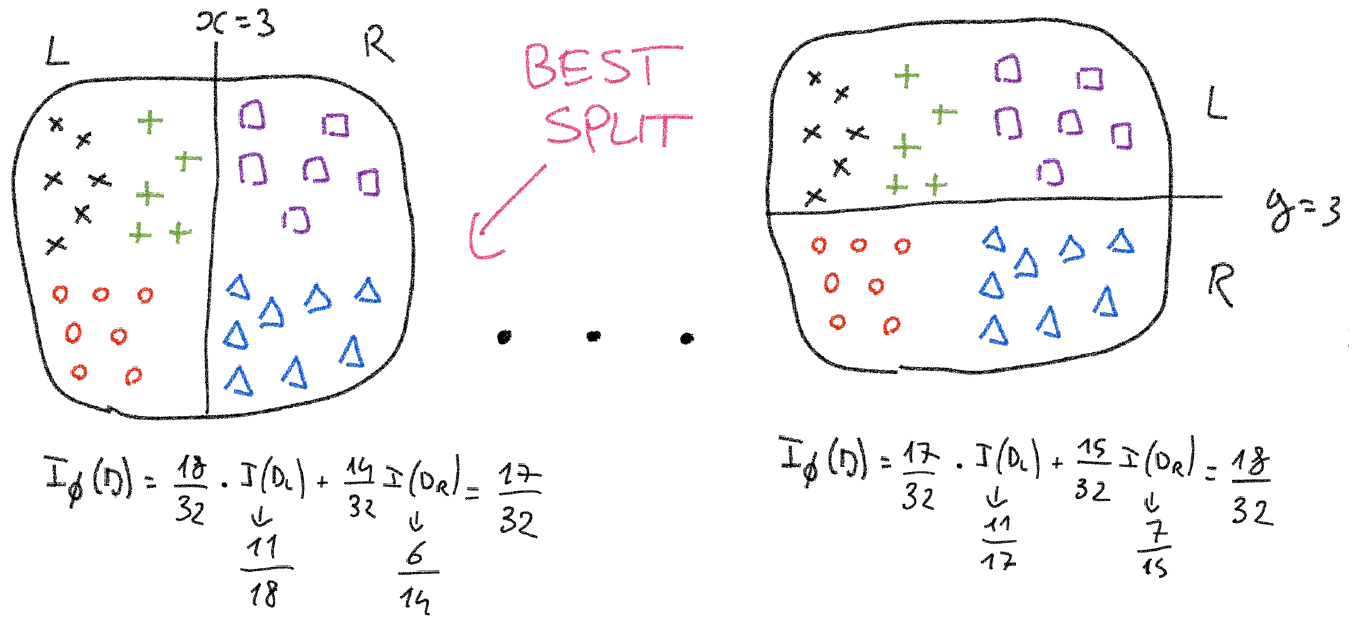
\includegraphics[width=1\linewidth]{imgs/chapter5/img10}
			\caption{Scelta dello split migliore}
			\label{fig:chapter05-10}
		\end{minipage}
	\end{figure}
	
	\begin{figure}
		\centering
		\begin{minipage}{.5\textwidth}
			\centering
			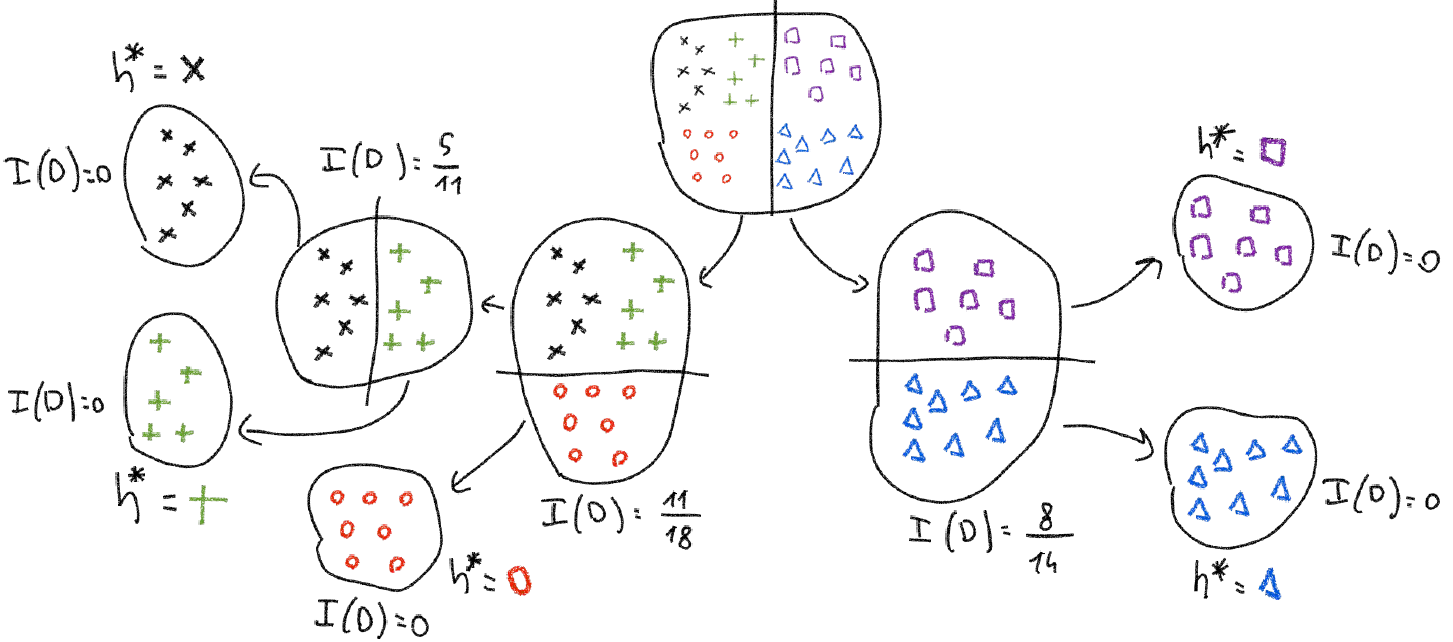
\includegraphics[width=1\linewidth]{imgs/chapter5/img11}
			\caption{Risultato finale}
			\label{fig:chapter05-11}
		\end{minipage}%
		\begin{minipage}{.5\textwidth}
			\centering
			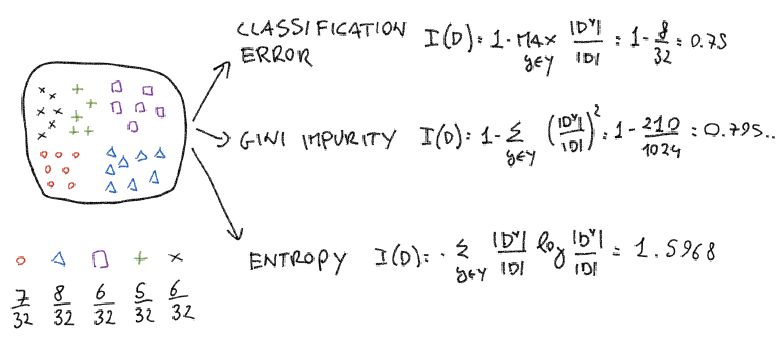
\includegraphics[width=1\linewidth]{imgs/chapter5/img5}
			\caption{Esempio misure di impurit\`a per la classificazione}
			\label{fig:chapter05-05}
		\end{minipage}
	\end{figure}

\section{Misure di impurit\`a per la regressione}
Si consideri per la regressione:
$$\mathcal{Y}\subset\mathbb{R}^d\qquad\qquad\qquad\mathcal{D}\subset\mathcal{X}\times\mathcal{Y}$$
Se $l(f;(x,y))=||f(x)-y||^2$ e $\mathcal{H}_{leaf} = \bigcup\limits_{y\in\mathcal{Y}}\{y\}^\mathcal{X}$ allora la misura di impurit\`a \`e la varianza:
$$I(\mathcal{D})=\dfrac{1}{|\mathcal{D}|}\sum\limits_{(x,y)\in\mathcal{D}}||x-\mu_\mathcal{D}||^2$$
Dove $\mu_\mathcal{D} = \frac{1}{|\mathcal{D}|}\sum\limits_{(x,y)\in\mathcal{D}}x$

\section{Data features e attributi}
Un data point $x\in\mathcal{X}$ potrebbe essere $d$ dimensionale con ogni dimensione con tipi di valori eterogenei come discreti o continui e avere un ordinamento o no, rispettivamente ordinali o nominali \ref{fig:chapter05-06}.

\begin{figure}
	\centering
	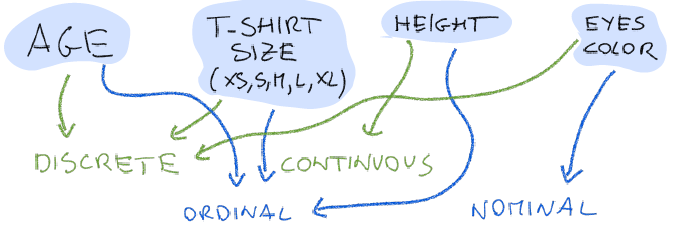
\includegraphics[width=0.6\linewidth]{imgs/chapter5/img6}
	\caption{Data features e attributi}
	\label{fig:chapter05-06}
\end{figure}

\section{Funzioni di split o routing}
Il routing o split $\phi\in\{L,R\}^{\mathcal{X}}$ determina se un data point $x\in\mathcal{X}$ deve muoversi a destra (i.e. $\phi(x)=\mathcal{R}$) o sinistra (i.e. $\phi(x)=\mathcal{L}$).
La possibile funzione di split \`e ristretta in un insieme predefinito $\Phi\subset\{L,R\}^\mathcal{X}$ in base alla natura dello spazio di features.
La funzione di split prototipica per un input $d$ dimensionale prima seleziona una dimensione e poi applica un criterio di split $1$ dimensionale.

	\subsection{Features discrete e nominali}
	Si assumano features discrete e nominali con valori in $\mathcal{K}$.
	La funzione di split pu\`o essere implementata data una partizione di $\mathcal{K}$ in $\mathcal{K}_R$ e $\mathcal{K}_L$:
	$$\phi(x) = \begin{cases}L &\mathbf{if} x\in\mathcal{K}_L\\
		R &\mathbf{if} x\in\mathcal{K}_R
	\end{cases}$$
	Trovare lo split ottimale richiede testare $2^{|\mathcal{K}|-1}-1$ bi-partizioni.
	
	\subsection{Features ordinali}
	Si assumano features ordinali con valori in $\mathcal{K}$.
	La funzione di split pu\`o essere implementata dando una soglia $r\in\mathcal{K}$:
	$$\phi(x) = \begin{cases}L &\mathbf{if} x\le r\\
		R &\mathbf{if} x>r
	\end{cases}$$
	Se $|\mathcal{K}|\le|\mathcal{D}|$ trovare lo split ottimale richiede il test di $|\mathcal{K}|-1$ soglie.
	Se $|\mathcal{K}|>|\mathcal{D}|$ si deve ordinare i valori di input in $\mathcal{D}$ dove $\mathcal{D}$ \`e il training set che raggiunge il nodo e testare $|\mathcal{D}|-1$ soglie.
	
	\subsection{Obliquo}
	A volte \`e conveniente fare split considerando pi\`u features alla volta.
	Tali funzioni lavorano con features continue e sono dette oblique in quanto generano decision boundaries obliqui.
	Se $x\in\mathbb{R}^d$ allora la funzione di split pu\`o essere implementata dato $w\in\mathbb{R}^d$ e $r\in\mathbb{R}$:
	$$\phi(x) = \begin{cases}L &\mathbf{if} w^Tx\le r\\
		R &\mathbf{altimenti}
	\end{cases}$$
	Si nota come questa funzione sia pi\`u difficile da ottimizzare.
	
	\section{Decision trees e overfitting}
	I decision trees sono modelli non parametrici con una struttura determinata dai dati.
	Per questo sono flessibili e possono facilmente fare fit sul training set, con un alto rischio di overfitting.
	Tecniche standard per migliorare la generalizzazione si applicano ai decision trees:
	\begin{multicols}{2}
		\begin{itemize}
			\item Early stopping.
			\item Regularization.
			\item Data augmentation.
			\item Complexity reduction.
			\item Ensembling.
		\end{itemize}
	\end{multicols}
	Una tecnica per ridurre la complessit\`a a posteriori \`e detta pruning.
	Se abbiamo un gran numero di attributi, possiamo trovare regolarità senza senso nei dati. 
	Oppure possiamo rimuovere anche gli attributi irrilevanti (processo manuale - non sempre possibile).

\section{Random forest}
Le random forest sono ensembles di decision trees \ref{fig:chapter05-08}.
Ogni albero \`e tipicamente trained con una versione bootstrapped del training set campionata con sostituzione.
Le funzioni di split sono ottimizzate su features campionate a caso o completamente a caso (extremely randomized trees).
Questo aiuta ad ottenere decision trees decorrelati.
La predizione finale della foresta \`e ottenuta facendo la media delle predizioni per ogni albero nell'ensemble $\mathcal{Q}=\{t_1,\dots,t_T\}$.
$$f_\mathcal{Q}(x)=\dfrac{1}{T}\sum\limits_{j=1}^Tf_t(x)$$

\begin{figure}
	\centering
	\begin{minipage}{.5\textwidth}
		\centering
		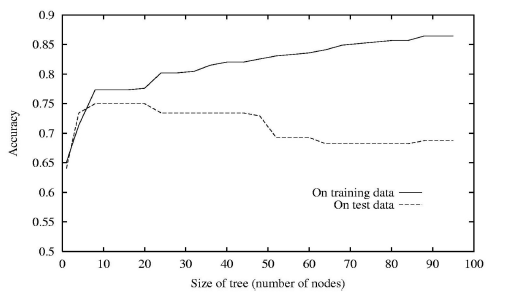
\includegraphics[width=1\linewidth]{imgs/chapter5/img7}
		\caption{Decision trees e overfitting. Aumentare il numero di nodi sui dati di training sembrava una buona idea quando non lo era sui dati di test.}
		\label{fig:chapter05-07}
	\end{minipage}%
	\begin{minipage}{.5\textwidth}
		\centering
		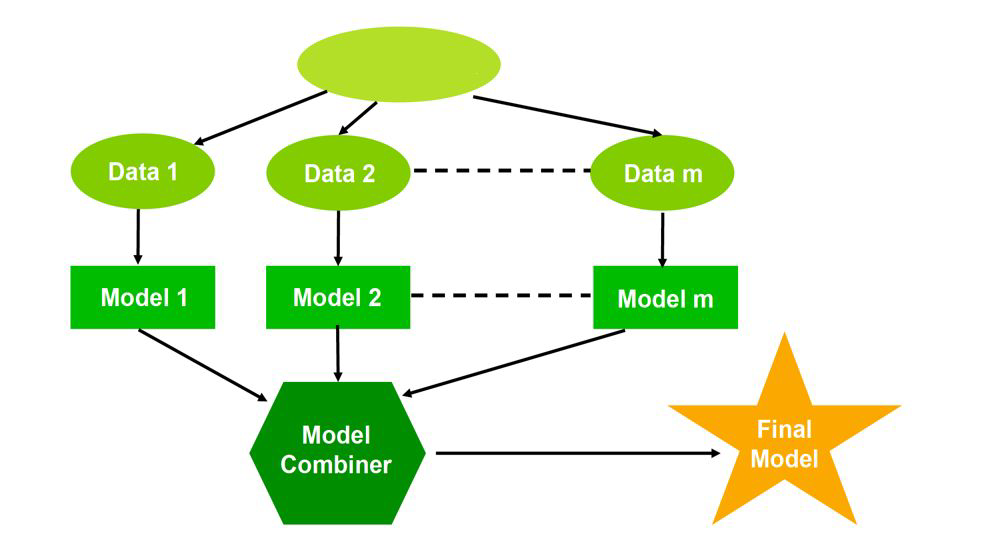
\includegraphics[width=1\linewidth]{imgs/chapter5/img8}
		\caption{Ensemble learning.}
		\label{fig:chapter05-08}
	\end{minipage}
\end{figure}

\section{Confronto con KNN}
Si nota come a differenza dei decision trees KNN non richiede nessun training, ma la classificazione \`e pi\`u veloce per i decision trees in quanto KNN per ogni esempio deve calcolare $k$ distanze.
A differenza di KNN che tratta tutte le features in maniera uguale i decision trees permettono una selezione delle features pi\`u importanti facendo scelte pesate.

	\chapter{Multi class classification}

\section{Introduzione}

	\subsection{Classificazione binaria}
	Si \`e definita la classificazione binaria come la task in cui dati:
	\begin{multicols}{2}
		\begin{itemize}
			\item Uno spazio di input $\mathcal{X}$.
			\item Una distribuzione sconosciuta $\mathcal{D}$ su $\mathcal{X}\times\{-1,+1\}$.
			\item Un training set $D$ campionato da $\mathcal{D}$
		\end{itemize}
	\end{multicols}
	Si deve computare una funzione $f$ che minimizza $\mathbb{E}_{(x,y)\sim\mathcal{D}}[f(x)\neq y]$

	\subsection{Classificazione multi classe}
	La classificazione multiclasse \`e l'estensione naturale della classificazione binaria.
	L'obiettivo \`e quello di assegnare una label discreta a degli esempi.
	La differenza \`e che ora ci sono $k>2$ classi da cui scegliere.
	Dati pertanto:
	\begin{multicols}{2}
		\begin{itemize}
			\item Uno spazio di input $\mathcal{X}$ e un numero di classi $K$.
			\item Una distribuzione sconosciuta di $\mathcal{D}$ su $\mathcal{X}\times[K]$.
			\item Un training set $D$ campionato da $\mathcal{D}$.
		\end{itemize}
	\end{multicols}
	Si deve computare una funzione $f$ che minimizza $\mathbb{E}_{(x,y)\sim\mathcal{D}}[f(x)\neq y]$.

		\subsubsection{K nearest neighbours}
		Si noti come una \emph{K-NN} per classificare un esempio $d$ trova i $k$ vicini di $d$ e sceglie la label in presenza maggiore tra i $k$ vicini pi\`u prossimi.
		Non necessita pertanto di cambi algoritmici nel caso della multi class classification.

		\subsubsection{Decision tree}
		I decision tree non richiedono cambi algoritmici per la multi class classification.

	\subsection{Approccio black box alla multi class classification}
	Dato un classificatore binario questo si pu\`o usare per risolvere il problema della multiclass classification.
	Si noti come un perceptron oltre al risultato pu\`o anche dare un punteggio di confidenza.
	Inoltre siccome una linea non \`e sufficiente per dividere le classi se ne possono usare diverse.

\section{One versus all \emph{OVA}}
Nell'approccio \emph{OVA} nel training si definisce per ogni label $L$ un problema binario in cui:
\begin{multicols}{2}
	\begin{itemize}
		\item Tutti gli esempi con la label $L$ sono positivi.
		\item Tutti gli altri esempi sono negativi.
	\end{itemize}
\end{multicols}
In pratica si imparano $L$ diversi modelli di classificazione.
Si ricordi come il classificatore divide il piano in due semipiani.

	\subsection{Ambiguit\`a}
	In questo caso si formano pertanto delle zone in cui si creano delle ambiguit\`a.
	Se il classificatore non fornisce confidence e c'\`e ambiguit\`a si sceglie una delle label in conflitto.
	Nella maggior parte dei casi i classificatori forniscono confidence, allora in questo caso si:
	\begin{multicols}{2}
		\begin{itemize}
			\item Si sceglie il positivo con confidence maggiore.
			\item Se nessuno \`e positivo si sceglie il negativo con confidence minore.
		\end{itemize}
	\end{multicols}
	La confidence nel perceptron si calcola come distanza dall'iperpiano stabilito dalla prediction.

	\subsection{Algoritmi}
	
\begin{algorithm}
\DontPrintSemicolon
\SetKwComment{comment}{$\%$}{}
\SetKw{Int}{int}
\SetKw{To}{to}
\SetKw{IsNot}{is not}
\SetKw{Not}{not}
\SetKw{Return}{Return}
\SetKwData{Item}{item}
\SetKwFunction{BinaryTrain}{BinaryTrain}
\SetKwFunction{Ova}{OneVersusAllTrain}

\caption{\protect\Ova{$D^{multiclass}$, \protect\BinaryTrain{}}}

\For{$i\ =\ 1$ \To $K$}{
	$D^{bin}$ = relabel $D^{multiclass}$ in modo che $i$ \`e positivo e $\neq i$ \`e negativo\;
	$f_i$ = \BinaryTrain{$D^{bin}$}\;
}
\Return $f_1,\dots, f_K$

\end{algorithm}

	\begin{algorithm}[H]
\DontPrintSemicolon
\SetKwComment{comment}{$\%$}{}
\SetKw{Int}{int}
\SetKw{To}{to}
\SetKw{IsNot}{is not}
\SetKw{Not}{not}
\SetKw{Return}{Return}
\SetKwData{Item}{item}
\SetKwFunction{BinaryTrain}{BinaryTrain}
\SetKwFunction{Ova}{OneVersusAllTest}
\SetKwFunction{Max}{max}

\caption{\protect\Ova{$f_1,\dots,f_K$, $\hat{x}$}}

score = $\langle 0,\dots, 0\rangle$		\comment{Inizializza $K$ score a $0$}

\For{$i\ =\ 1$ \To $K$}{
	y = $f_i(\hat{x})$\;
	$score_i\ =\ score_i + y$\;
}
\Return \Max{score}\;

\end{algorithm}


\section{All versus all \emph{AVA}}
Un approccio alternativo consiste nel gestire il problema della classificazione multi classe decomponendolo in problemi di classificazione binaria.
Questo approccio viene detto anche all pairs.
Si classificano $\frac{K(K-1)}{2}$ classificatori in modo che
$$F_{ij}, 1\le i< j \le K$$
Sia il classificatore che discrimina la classe $i$ contro la classe $j$.
Questo classificatore riceve tutti gli esempi della classe $i$ come positivi e tutti gli esempi della classe $j$ come negativi.
Quando arriva un punto di test si valuta su tutti i classificatori $F_{ij}$.
Ogni volta che $F_{ij}$ predice positivo la classe $i$ prende un voto, altrimenti lo prende $j$.
Dopo aver eseguito tutti i $\frac{K(K-1)}{2}$ classificatori la classe con pi\`u voti decide la label.

	\subsection{\emph{AVA} training}
	Per ogni coppia di label si addestra un classificatore che le distingue:
	\begin{algorithm}[H]
\DontPrintSemicolon
\SetKwComment{comment}{$\%$}{}
\SetKw{Int}{int}
\SetKw{To}{to}
\SetKw{IsNot}{is not}
\SetKw{Not}{not}
\SetKw{Return}{Return}
\SetKwData{Item}{item}
\SetKwFunction{BinaryTrain}{BinaryTrain}
\SetKwFunction{Ava}{AllVersusAllTrain}
\SetKwFunction{Max}{max}

\caption{\protect\Ava{}}
\For{i = 1 \To number of labels}{
	\For{j = i + 1 \To number of labels}{
		train a classifier $F_{ij}$ to distinguish between $label_j$ and $label_i$\;
		create a dataset with all examples with $label_j$ labeled positive and with $label_i$ negative\;
		Train classifier $F_{ij}$ su questo sottoinsieme di dati\;
	}
}
\end{algorithm}


	\subsection{\emph{AVA} classification}
	Per classificare un esempio $x$ lo si classifica per ogni classificatore $F_{ij}$.
	Per scegliere la classe finale si pu\`o:
	\begin{multicols}{2}
		\begin{itemize}
			\item Considerare la maggioranza.
			\item Considerare un voto pesato basato sulla confidence:
				\begin{itemize}
					\item $y = F_{ij}(x)$.
					\item $score_j +=y$.
					\item $score_i -=y$.
				\end{itemize}
				Lo score viene cambiato in quanto se $y$ \`e positivo il classificatore lo pensa di tipo $j$, se negativo lo pensa di tipo $i$ e pertanto lo score viene aggiornato di conseguenza.
		\end{itemize}
	\end{multicols}

	\subsection{Algoritmi}
	\begin{algorithm}
\DontPrintSemicolon
\SetKwComment{comment}{$\%$}{}
\SetKw{Int}{int}
\SetKw{To}{to}
\SetKw{IsNot}{is not}
\SetKw{Not}{not}
\SetKw{Return}{Return}
\SetKwData{Item}{item}
\SetKwFunction{BinaryTrain}{BinaryTrain}
\SetKwFunction{Ava}{AneVersusAllTrain}

\caption{\protect\Ava{$D^{multiclass}$, \protect\BinaryTrain{}}}
$f_{ij}\ =\ \emptyset,\ \forall 1\le i < j \le K$\;
\For{$i\ =\ 1$ \To $K\ -\ 1$}{
	$D^{pos}\ =\ $ all $x\in D^{multiclass}$ labeled $i$\;
	\For{$j\ =\ j\ +\ 1$ \To $K$}{
		$D^{neg}\ =$ all $x\in D^{multiclass}$ labeled $j$\;
		$D^{bin}\ =\ \{(x, +1):x\in D^{pos}\}\cup\{(x,-1):x\in D^{neg}\}$\;
		$f_{ij}$ = \BinaryTrain{$D^{bin}$}\;
	}
}

\Return all $f_{ij}$

\end{algorithm}

	\begin{algorithm}[H]
\DontPrintSemicolon
\SetKwComment{comment}{$\%$}{}
\SetKw{Int}{int}
\SetKw{To}{to}
\SetKw{IsNot}{is not}
\SetKw{Not}{not}
\SetKw{Return}{Return}
\SetKwData{Item}{item}
\SetKwFunction{BinaryTrain}{BinaryTrain}
\SetKwFunction{Ava}{AllVersusAllTest}
\SetKwFunction{Max}{max}

\caption{\protect\Ava{all $f_{ij}$, $\hat{x}$}}

score = $\langle 0,\dots, 0\rangle$		\comment{Inizializza $K$ score a $0$}

\For{$i\ =\ 1$ \To $K\ -\ 1$}{
	\For{$j\ =\ i\ +\ 1$ \To $K$}{
		y = $f_{ij}(\hat{x})$\;
		$score_i\ =\ score_i + y$\;
		$score_j\ =\ score_j - y$\;
	}
}
\Return \Max{score}\;

\end{algorithm}


\section{Confronto tra \emph{OVA} e \emph{AVA}}

	\subsection{Tempo di training}
	\emph{AVA} impara pi\`u classificatore ma il training set \`e omlto pi\`u piccolo pertanto tende ad essere pi\`u veloce se le label sono equamente bilanciate.

	\subsection{Tempo di test}
	Avendo \emph{AVA} pi\`u classificatori \`e tipicamente pi\`u lenta.

	\subsection{Errori}
	\emph{AVA} fa training con data sets pi\`u bilanciata, ma avendo pi\`u classificatori i test tendono ad avere pi\`u possiblit\`a di errori.

\section{Riassunto}
Se vengono usati classificatori binari viene tipicamente utilizzata  \emph{OVA}, altrimenti si usa un classificatore che permette label multiple come \emph{DT} o \emph{K-NN}, nonostante altri metodi pi\`u sofisticati siano meglio.

\section{Multiclass evaluation}

	\subsection{Microaveraging}
	Nel microaveraging si fa la media sugli esempi.

	\subsection{Macroaveraging}
	Nel macroaveraging si calcola lo score di valutazione o accuratezza per ogni label e poi si fa la media tra le label.
	Questo in quanto d\`a pi\`u enfasi a label pi\`u rare e permette un'altra dimensione di analisi.

	\subsection{Confusion matrix}
	La confusion matrix \`e una matrice in cui $(i, j)$ rappresenta il numero di esempi con label $i$ predetti avere label $j$.
	Viene spesso espressa come percentuale.

	\chapter{Gradient descent}

\section{Model based machine learning}
Nel model based machine learning si sceglie un modello definito da un insieme di parametri.
In particolare si nota come:
\begin{multicols}{2}
	\begin{itemize}
		\item Per i decision trees i parametri sono la struttura dell'albero, quali features ogni nodo divide e le predizioni delle foglie.
		\item Per il perceptron i parametri sono i pesi e il valore di $b$.
	\end{itemize}
\end{multicols}
Dopo aver scelto il modello si deve scegliere un criterio da ottimizzare o la funzione obiettivo come per esempio il training error.
Infine si sviluppa un algoritmo di learning che deve cercare di minimizzare il criterio, spesso in maniera euristica.

	\subsection{Modelli lineari}
	Nei modelli lineari il modello \`e:
	$$0=b+\sum\limits_{j=1}^mw_jf_j$$
	Si deve scegliere il criterio da ottimizzare.

		\subsubsection{Notazioni}

			\paragraph{Funzione indicatrice}
			Una funzione indicatrice trasforma valori di \emph{Vero} e \emph{Falso} in numeri e conte.
			$$1[x]=\begin{cases}1&\mathbf{if} x = True\\
										  	0&\textbf{if} x = False
				 	\end{cases}$$

			\paragraph{Dot-product}
			Utilizzando una notazione vettoriale si rappresenta un esempio $f_1,\dots,f_m$ come un vettore singolo $\overrightarrow{x}$ in cui $j$ indicizza la feature e $i$ indicizza un dataset di esempi.
			Si possono rappresentare anche i pesi $w_1,\dots,w_m$ come un vettore $\overrightarrow{w}$.
			Il dot-product tra due vettori $a$ e $b$ viene definito come:
			$$a\cdot b = \sum\limits_{j=1}^ma_jb_j$$

		\subsubsection{Funzione obiettivo}
		Il criterio da ottimizzare o funzione obiettivo pu\`o essere:
		$$\sum\limits_{i=1}^n1[y_i(w\cdot x_i+b)\le 0]$$
		Si devono pertanto trovare $w$ e $b$ tali che minimizzano questa funzione, ovvero:
		$$argmin_{w,b}\sum\limits_{i=1}^n1[y_i(w\cdot x_i+b)\le 0]$$

\section{Loss functions}

	\subsection{Loss $0/1$}
	Una funzione di loss $0/1$ \`e una funzione nella forma:
	$$\sum\limits_{i=1}^n1[y_i*w\cdot x_i+b)\le 0]$$
	Dove tra le quadre si trova se la predizione e la label sono d'accordo, con vero se non lo fanno e tra le tonde la distanza dall'iperpiano, di cui il segno \`e la predizione.
	Questa funzione ritorna il numero di sbagli.

		\subsubsection{Minimizzare la loss $0/1$}
		Per minimizzare una funzione $0/1$ si deve, ogni volta cambiare un valore di $w$ in modo che l'esempio \`e corretto o scorretto la perdita aumenta o diminuisce.
		Si nota come a ogni feature aggiunta si aggiunge una nuova dimensione allo spazio.
		Il minimo si trova trovando $w$ e $b$ che minimizzano la perdita.
		Questo \`e un problema \emph{NP-hard}.
		Sue difficolt\`a comprendono il fatto che piccoli cambi in ogni $w$ possono portare a grandi cambi nella perdita in quanto il cambio non \`e continuo.
		Ci possono essere molti minimi locali.
		Ad ogni punto non si hanno informazioni che direzionano verso il minimo.
		Pertanto si nota come una loss function ideale sia continua e differenziabile in modo da avere un'indicazione verso la direzione di minimizzazione e un unico minimo.

	\subsection{Funzioni convesse}
	In una funzione convessa il segmento tra qualsiasi due punti della funzione si trova al di sopra della funzione.

	\subsection{Surrogate loss function}
	Per molte applicazioni si vuole minimizzare la loss $0/1$.
	Una surrogate loss function \`e una loss function che fornisce un limite superiore alla loss function attuale.
	Si vuole identificare un surrogato convesso della loss function in modo da facilitarne la minimizzazione.
	Chiave a una loss function \`e come verifica la differenza tra la label $y$ effettiva e la predizione $y'$.

		\subsubsection{Alcune surrogate loss function}
		\begin{multicols}{2}
			\begin{itemize}
				\item \emph{$01$ loss}: $l(y, y')=1[yy'\le 0]$.
				\item \emph{Hinge} $l(y,y')=\max(0,1-yy')$.
				\item Exponential: $l(y,y')=\exp(iyy')$
				\item \emph{Squared loss}: $l(y,y')=(y-y')^2$.
			\end{itemize}
		\end{multicols}

\section{Gradient descent}
Il gradient descent \`e un modo per trovare il minimo di una funzione: le derivate parziali danno un slope o direzione dove muoversi in tale dimensione.
Questo approccio consiste di scegliere un punto di partenza e a ripetizione di: scegliere una dimensione e muoversi di una piccola quantit\`a verso il minimo utilizzando la derivata.

	\subsection{Spostamento in direzione della minimizzazione dell'errore}
	Il movimento in direzione della minimizzazione dell'errore \`e pertanto:
	$$w_j = w_j - \eta \dfrac{d}{dw_i}loss(w)$$
	Dove $\eta$ \`e il learning rate.

		\subsubsection{Calcolo dello spostamento per la loss function esponenziale}
		Si deve pertanto calcolare:
		\begin{align*}
			\dfrac{d}{dw_j}loss &=\dfrac{d}{dw_j}\sum\limits_{i=1}^n\exp(-y_i(w\cdot x_i + b))\\=
												 &=\sum\limits_{i=1}^n\dfrac{d}{dw_j}[-y_i(w\cdot x_i+b)]\exp(-y_i(w\cdot x_i+b))\\
		\end{align*}
		Si consideri pertanto ora:
		\begin{align*}
			\dfrac{d}{dw_j}[-y_i(w\cdot x_i + b)]&=-\dfrac{d}{dw_j}[-y_i(w\cdot x_i + b)]=\\
																		&=-\dfrac{d}{dw_j}y_i(w_1x_{i1}+\cdots+w_mx_{im}+b)=\\
																		&=-y_ix_{ji}
		\end{align*}
		Si nota pertanto come:
		$$\dfrac{d}{dw_j}loss=\sum\limits_{i=1}^n-y_ix_{ij}\exp(-y_i(w\cdot x_i+b))$$
		Si aggiorna pertanto $w_j$:
		$$w_j=w_j-\eta\sum\limits_{i=1}^n-y_ix_{ij}\exp(-y_i(w\cdot x_i+b))$$
		Questo viene fatto per ogni esempio $x_i$.

	\subsection{Learning algorithm del perceptron}
	Si nota pertanto come considerando il perceptron nell'ambito del gradient descent si aggiorna sempre il vettore dei pesi.
	\begin{algorithm}[H]
\DontPrintSemicolon
\SetKwComment{comment}{$\%$}{}
\SetKw{Int}{int}
\SetKw{To}{to}
\SetKw{IsNot}{is not}
\SetKw{Not}{not}
\SetKwData{Item}{item}
\SetKwFunction{Min}{min}
\SetKwFunction{Perceptron}{Perceptron}

\caption{\protect\Perceptron{}}

\Repeat{Convergence}{
	\ForEach{training example ($f_1, f_2,\dots,f_n, label$)}{
		\comment{Label = $\pm 1$}
		$prediction\ =\ b\ +\ \sum\limits_{i=1}^nw_if_i$\;
			\ForEach{$w_i$}{
				$w_j = w_j + \eta y_ix_{ij}\exp(-y_i(w\cdot x_i + b))$
				$b\ =\ b\ +\ label$\;
			}
		}
	}



\end{algorithm}

	Si noti come in questo caso $\eta$ rappresenta il learning rate, $y_i$ la label e $(w\cdot x_i + b))$ la predizione.
	Questi generano una costante $c$

	\subsection{Costante $\mathbf{c}$}
	Nella costante $c$ se label e predizione hanno lo stesso segno quando gli elementi predetti aumentano gli aggiornamenti diventano minori.
	Se invece sono diversi pi\`u diversi lo sono, maggiore l'aggiornamento.

	\subsection{Gradiente}
	Il gradiente \`e il vettore delle derivate parziali rispetto a tutte le coordinate dei pesi:
	$$\nabla L = \biggl[\dfrac{\delta L}{\delta w_1}\cdots\dfrac{\delta L}{\delta w_N}\biggr]$$
	Ogni derivata parziale misura quanto veloce la perdita cambia in una direzione.
	Quando il gradiente \`e zero la perdita non sta cambiando in nessuna direzione.
	
\begin{algorithm}
\DontPrintSemicolon
\SetKwComment{comment}{$\%$}{}
\SetKw{Int}{int}
\SetKw{To}{to}
\SetKw{IsNot}{is not}
\SetKw{Not}{not}
\SetKw{Return}{return}
\SetKwData{Item}{item}
\SetKwFunction{Min}{min}
\SetKwFunction{GradientDescent}i{GradientDescent}

\caption{\protect\GradientDescent{$\mathcal{F}$, $K$, $\eta_1$, $\dots$}}
	$z^{(0)}\ \rightarrow <0,0,\dots,0$\comment{Inizializza la variabile da ottimizzare}
	\For{$k = 1$ \To $K$}{
		$g^{(k)}\ \rightarrow\ \nabla_z\mathcal{F}|_{z^{(k-1)}}$\comment{Computa il gradiente nella posizione corrente}
		$z^{(k)} \rightarrow z^{(k-1)} - \eta^{(k)}g^{(k)}$\comment{scendi il gradiente}
	}
	\Return $z^{(k)}$\end{algorithm}

	Nei problemi in cui il problema di ottimizzazione \`e non convesso si trovano dei minimi locali, questi non permettono all'algoritmo di proseguire in quanto non distingue tra minimi locali e minimi globali.
	Un altro punto \`e un punto a sella, in cui certe direzioni curvano verso l'alto e altre verso il basso.
	In tali punti il gradiente \`e $0$ e l'algoritmo si blocca.
	Un modo per uscire da un punto \`a sella \`e spostarsi a lato un po' in modo da uscirne.
	Si nota come i punti a sella sono molti comuni in alte dimensioni.
	Il learning rate \`e molto importante in quanto permette di decidere la distanza coperta da uno spostamento determinando velocit\`a di avvicinamento al minimo e precisione dell'algoritmo.

	\chapter{Regularization}

\section{Introduzione}
Si noti come con il gradient descent si calcola il valore minimo della loss function sul training set.
Ci si deve pertanto preoccupare del overfitting.
Il minimo $w$ e $b$ sul training set infatti non sono tipicamente il minimo per il test set.
Questo problema viene risolto attraverso la regolarizzazione.

\section{Regolarizzatori}
I regolarizzatori sono criteri addizionali alla loss function in modo da evitare overfitting.
Prova a mantenere i parametri regolari o normali.
\`E un bias sul modello che forza che il learning preferisca certi tipi di pesi rispetto agli altri.
$$argmin_{w,b}\sum\limits_{i=1}^nloss(yyy')+\lambda regularizer(w,b)$$
Tipicamente non si vogliono pesi molto grandi in quanto un piccolo cambio in una feature potrebbe causare un cambio nella predizione.
Si potrebbe anche preferire pesi di $0$ per features che non sono utili.

	\subsection{Regolarizzatori comuni}

		\subsubsection{Somma dei pesi}
		Il regolarizza otre somma dei pesi penalizza di pi\`u piccoli valori e si calcola come:
		$$r(w,b)=\sum\limits_{w_j}|w_j|$$
		Si dice anche $1$-norm.

		\subsubsection{Somma quadratica dei pesi}
		La somma quadratica dei pesi penalizza di pi\`u valori grandi e si calcola come:
		$$r(w,b)=\sqrt{\sum\limits_{w_j}|w_j|^2}$$
		Si dice anche $2$-norm.

		\subsubsection{$P$-norm}
		Si intende per $p$-norm:
		$$r(w,b)=\sqrt[p]{\sum\limits_{w_j}|w_j|^p}=||w||^p$$
		Valori pi\`u piccoli di $p$ $<2$ incoraggiano vettori pi\`u sparsi, mentre valori pi\`u grandi scoraggiano pesi pi\`u grandi creando pertanto vettori con pesi pi\`u simili.

\section{Gradient descent e regolarizzazione}
Si nota come se scelto un modello e dimostrato che $loss+regularizer$ \`e una funzione convessa si pu\`o ancora utilizzare il gradient descent.
Si nota come per costruzione le $p$-norms sono convesse per $p\ge 1$ e pertanto:
\begin{align*}
	\dfrac{d}{dw_j}objective&=\dfrac{d}{dw_j}\sum\limits_{i=1}^n\exp(-y_i(w\cdot x_i + b))+\dfrac{\lambda}{2}||w||^2=\\
				&\cdot\\
				&\cdot\\
				&\cdot\\
				&=-\sum\limits_{i=1}^ny_ix_{ij}\exp(-y_i(w\cdot x_i+b))+\lambda w_j
\end{align*}
Pertanto con il regolarizzatore l'aggornamento \`e
$$w_j=w_j+\eta y_ix_{ij}\exp(-y_i(w\cdot x_i+b))-\eta\lambda w_j$$
Si noti pertanto come la regolarizzazione, se $w_i$ \`e positiva la riduce, mentre se \`e negativa lo aumenta muovendo $w_i$ verso lo $0$.

\section{Regolarizzazione con le $p$-norms}

	\subsection{L1}
	$$w_j = w_j + \eta(lossCorrection - \lambda sign(w_j))$$
	Popolare in quanto tende a dare soluzioni sparse, ma non \`e differenziabile e lavora unicamente per risolutori a gradient descent.
		
	\subsection{L2}
	$$w_j = w_j + \eta(lossCorrection - \lambda w_j)$$
	Popolare in quanto per qualche loss function pu\`o essere risolta direttamente.

	\subsection{Lp}
	$$w_j = w_j + \eta(lossCorrection - \lambda cw_j^{p-1})$$
	Meno popolare in quanto non riduce i pesi abbastanza.

\section{Metodi di machine learning con regolarizzazione}
\begin{multicols}{2}
	\begin{itemize}
		\item Ordinario: least squares: squared loss.
		\item Ridge regression: squared loss with L2 regularization
		\item Lasso regression: squared loss with L1 regularization
		\item Elastic regression: squared loss with L2 and L1 regularization
		\item Logistic regression: logistic loss.
	\end{itemize}
\end{multicols}


\end{document}
